\documentclass[conf]{new-aiaa}
%\documentclass[journal]{new-aiaa} for journal papers
\usepackage[utf8]{inputenc}

\usepackage{graphicx}
\usepackage{amsmath}
\usepackage{commath}
\usepackage[version=4]{mhchem}
\usepackage{siunitx}
\usepackage{longtable,tabularx}
\usepackage{float}
\usepackage{listings}
\usepackage{pdfpages}
\usepackage{color} %red, green, blue, yellow, cyan, magenta, black, white
\definecolor{mygreen}{RGB}{28,172,0} % color values Red, Green, Blue
\definecolor{mylilas}{RGB}{170,55,241}
\setlength\LTleft{0pt} 

\lstset{language=Matlab,%
	basicstyle=\footnotesize,
	breaklines=true,%
	morekeywords={matlab2tikz},
	keywordstyle=\color{blue},%
	morekeywords=[2]{1}, keywordstyle=[2]{\color{black}},
	identifierstyle=\color{black},%
	stringstyle=\color{mylilas},
	commentstyle=\color{mygreen},%
	showstringspaces=false,%without this there will be a symbol in the places where there is a space
	numbers=left,%
	numberstyle={\tiny \color{black}},% size of the numbers
	numbersep=9pt, % this defines how far the numbers are from the text
	emph=[1]{for,end,break},emphstyle=[1]\color{red}, %some words to emphasise
	%emph=[2]{word1,word2}, emphstyle=[2]{style},    
}

% ================================================================ % 
\title{ASE 381.P3 Optimal Control Theory \\ Homework 2}

\author{Junette Hsin}
\affil{Masters Student, Aerospace Engineering and Engineering Mechanics, University of Texas, Austin, TX 78712}

\begin{document}

\maketitle

% \begin{abstract}

	% The theory and algorithms are derived and computer program to establish the trajectory of
	% an Earth-orbiting satellite is developed. The assumptions for the study are ...

% \end{abstract}


% ================================================================ % 
\section*{Problem 1}

% Statement 
\begin{center}
	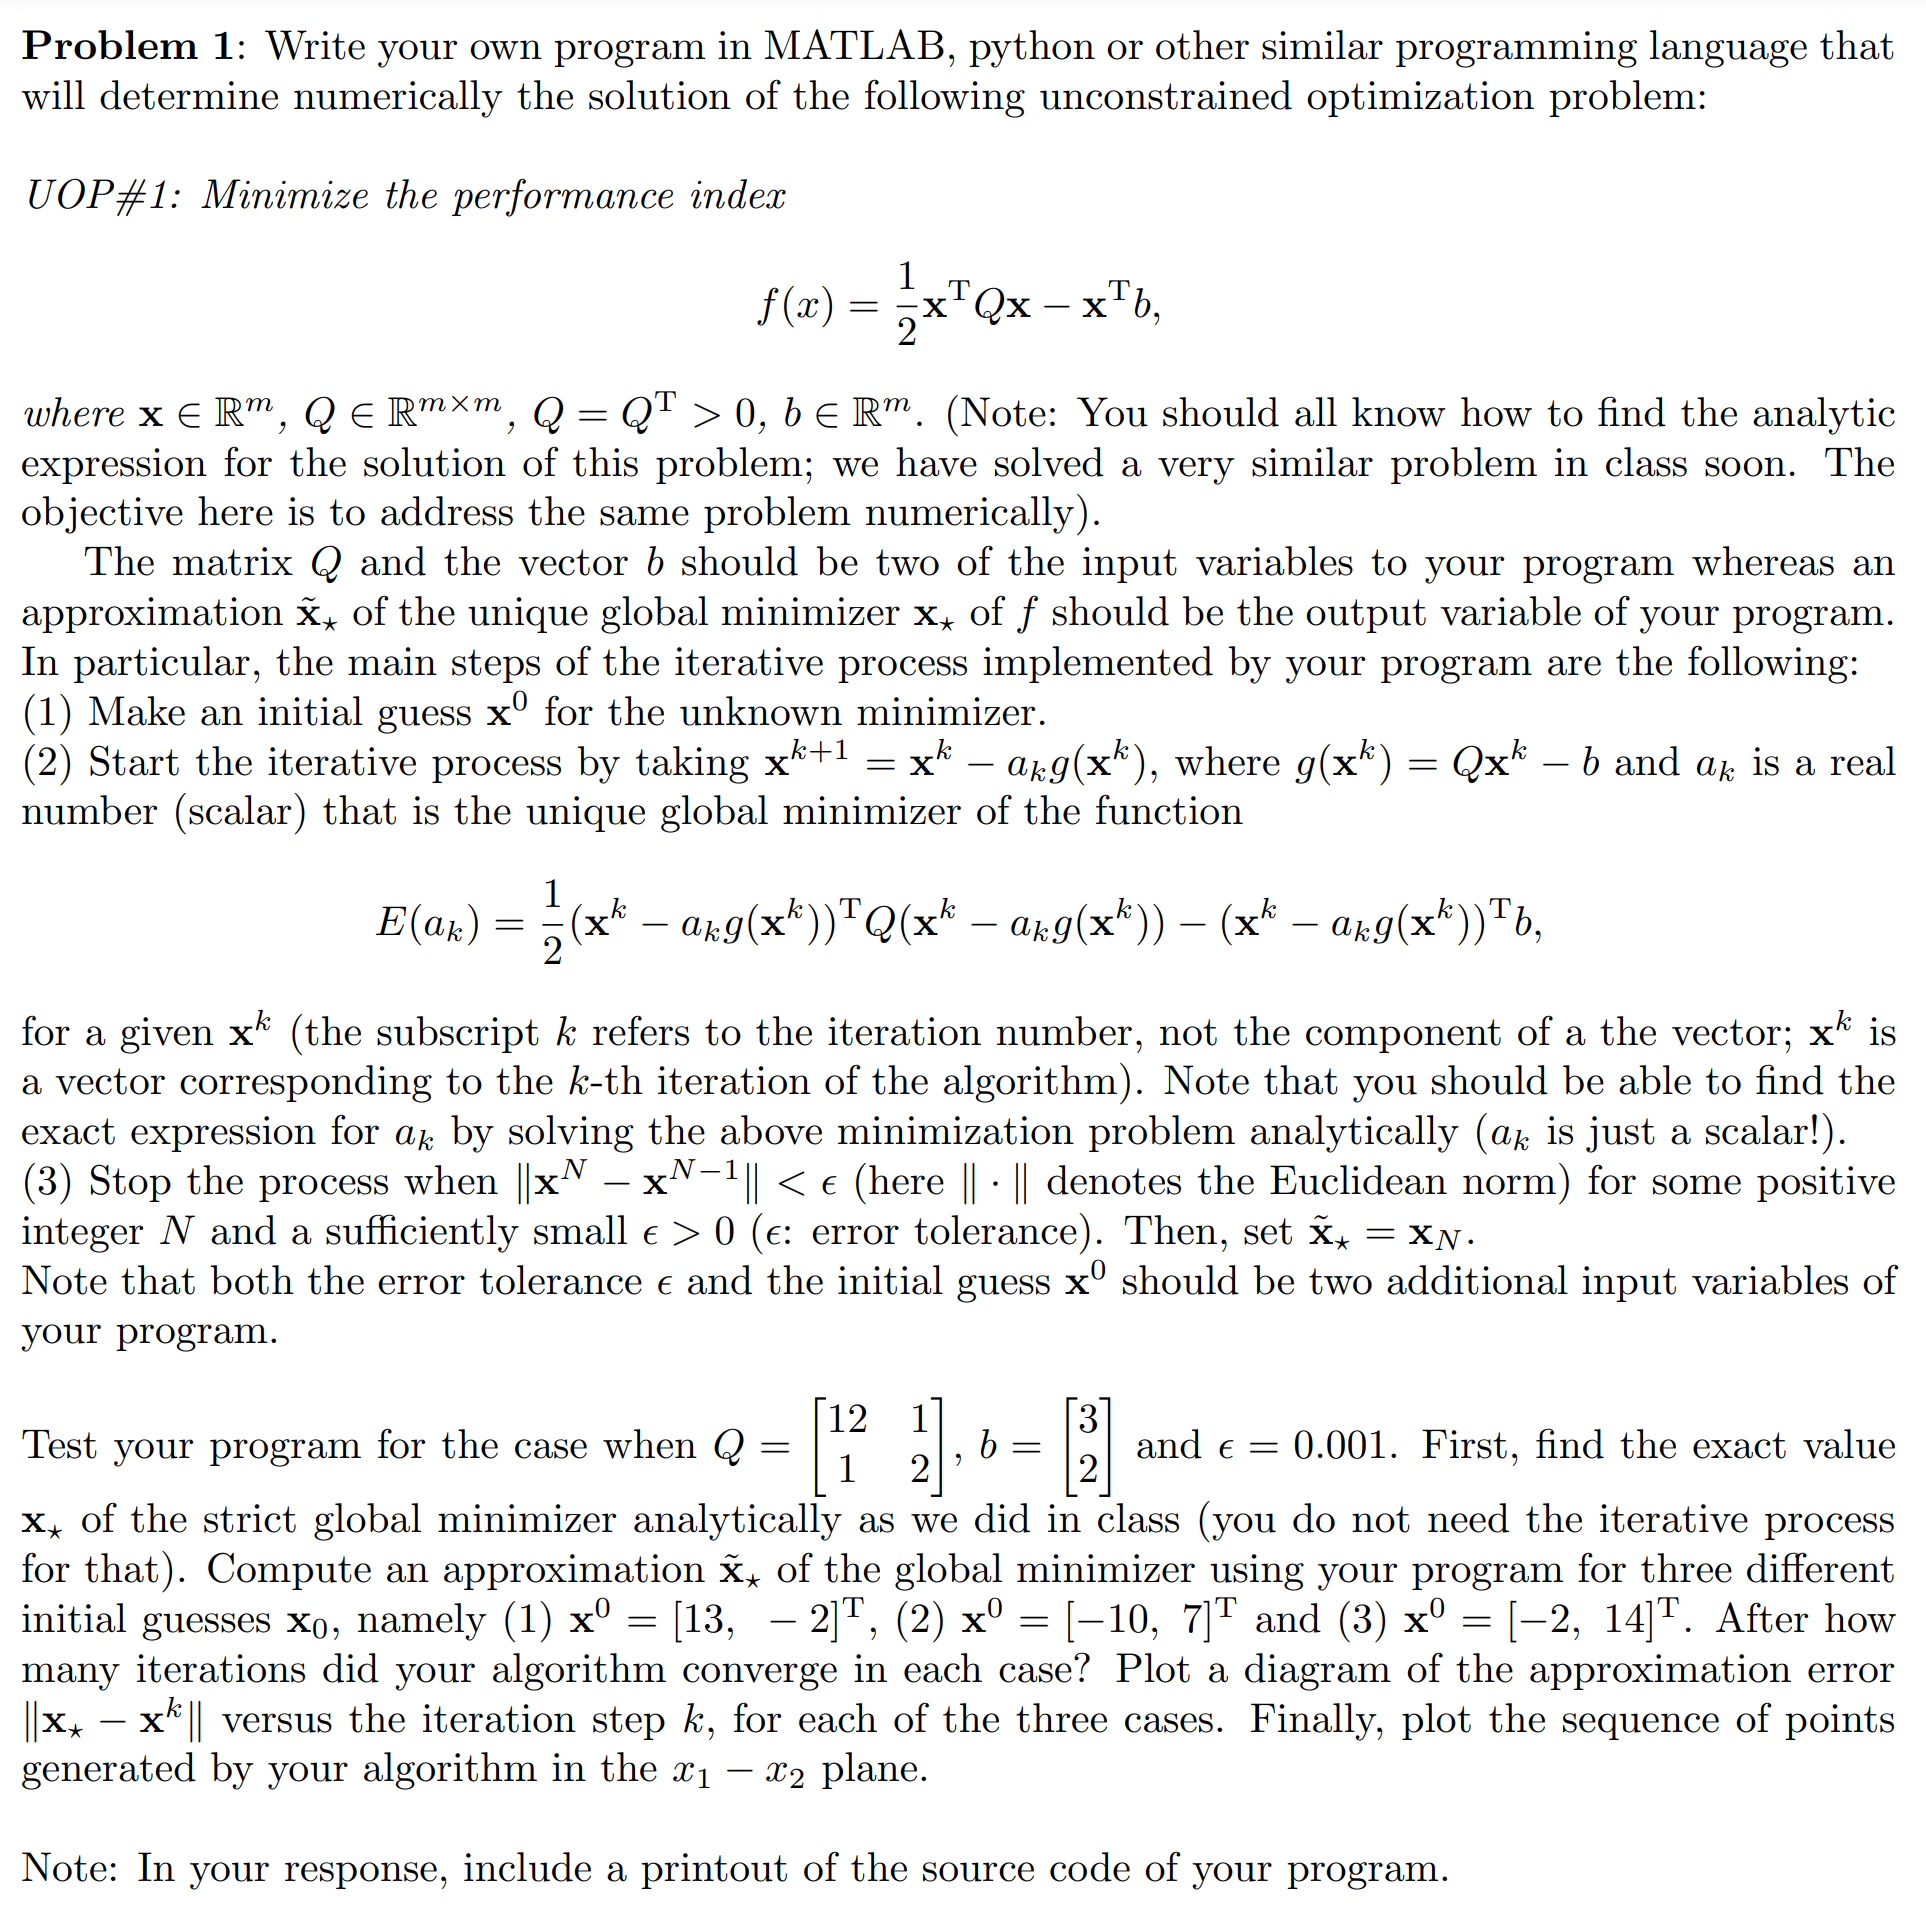
\includegraphics[width=0.9\textwidth]{P1.png}
\end{center}

\newpage 

% Solution 

% PART ONE 
\subsection{Solution}

The analytical solution for the strict global minimizer for all 3 cases is $x_* = [0.173913043478261, 0.91304347826087 ]$. 

The unique global minimizer $a_k$ was found analytically by differentiating $E(a_k)$ with respect to $a_k$, which resulted in the following expression: 

\begin{equation}
	a_{k *} = [x_k^T Q g_k - g_k^T b] [g_k^T Q g_k]^{-1}
\end{equation}

Code specific to each of the 3 cases are located in their individual sections, but additional functions and code required for each algorithm can be found in the Appendix. 


\subsection{Case 1: x$^0$ = [13, -2]$^T$}

\subsubsection{Plots}

\begin{figure}[H]
	\begin{center}
		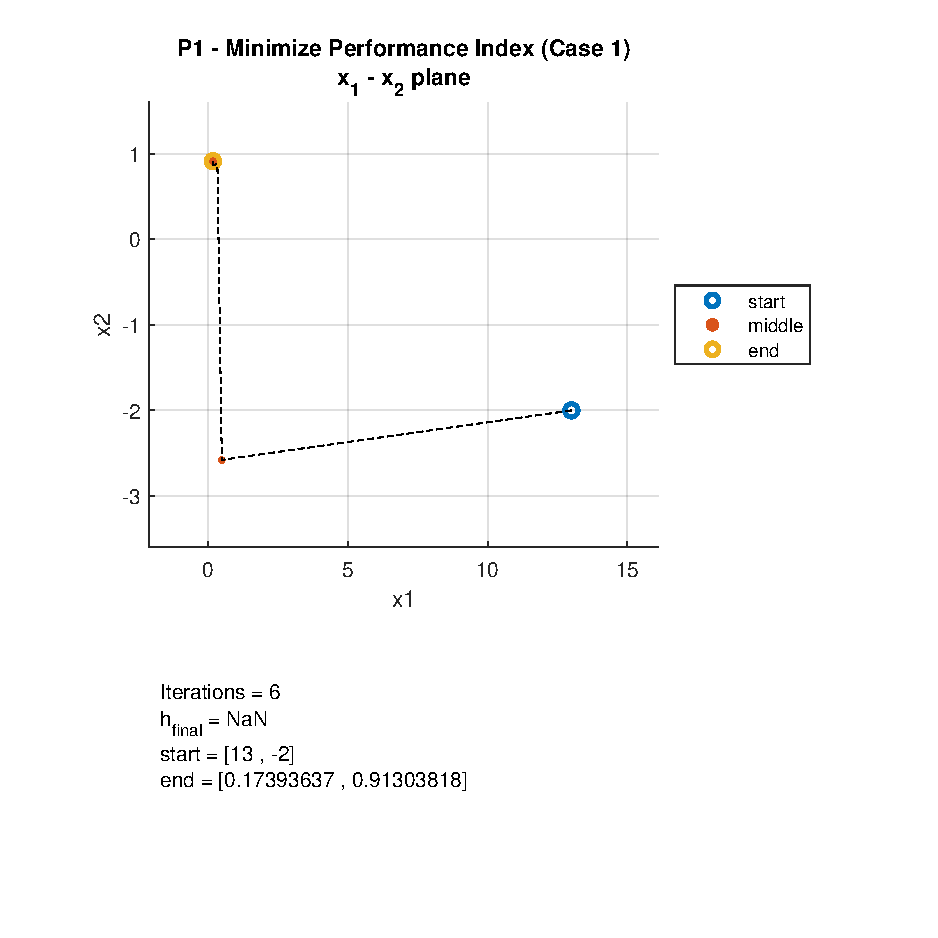
\includegraphics[width=0.9\textwidth]{P1 - Minimize Performance Index (Case 1) - x_1 - x_2 plane.pdf}
	\end{center}
	\caption{Problem 1: Case 1: x1-x2 plane}
\end{figure}

The algorithm took 6 iterations to converge below the threshold $\epsilon = 0.001$. 

\begin{figure}[H]
	\begin{center}
		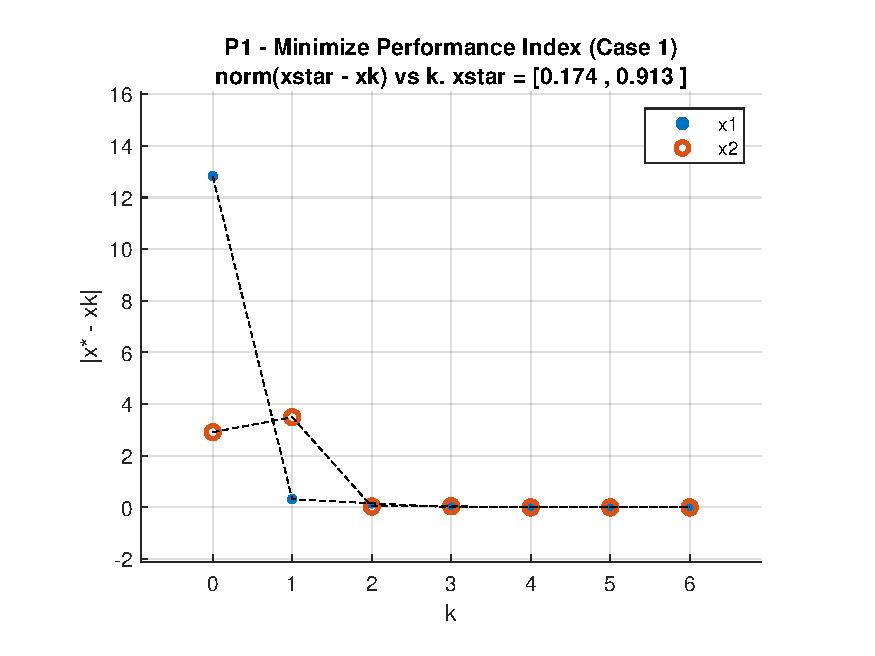
\includegraphics[width=0.8\textwidth]{P1 - Minimize Performance Index (Case 1) - norm(xstar - xk) vs k. xstar = [0.174 , 0.913 ].pdf}
	\end{center}
	\caption{Problem 1: Case 1: Iteration vs. Error}
\end{figure}

% PART TWO 
\subsection{Case 2: x$^0$ = [-10, 7]$^T$}

\subsubsection{Plots}

\begin{figure}[H]
	\begin{center}
		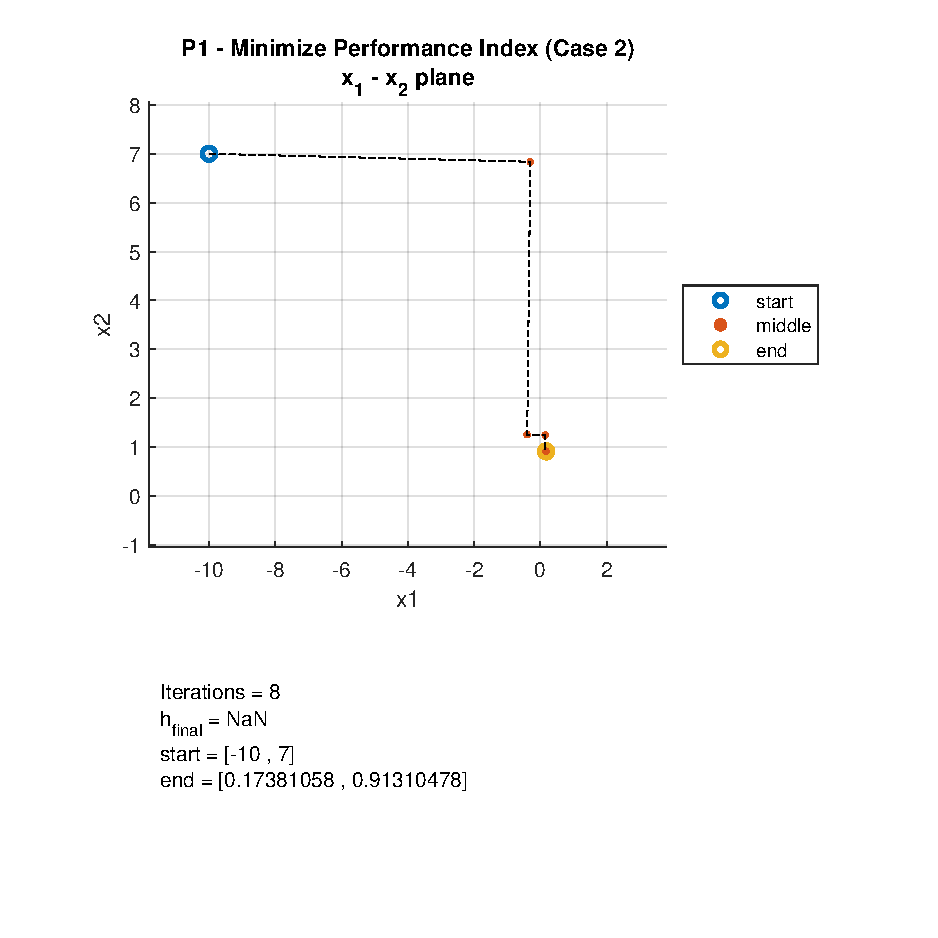
\includegraphics[width=0.9\textwidth]{P1 - Minimize Performance Index (Case 2) - x_1 - x_2 plane.pdf}
	\end{center}
	\caption{Problem 1: Case 2: x1-x2 plane}
\end{figure}

The algorithm took 8 iterations to converge below the threshold $\epsilon = 0.001$. 

\begin{figure}[H]
	\begin{center}
		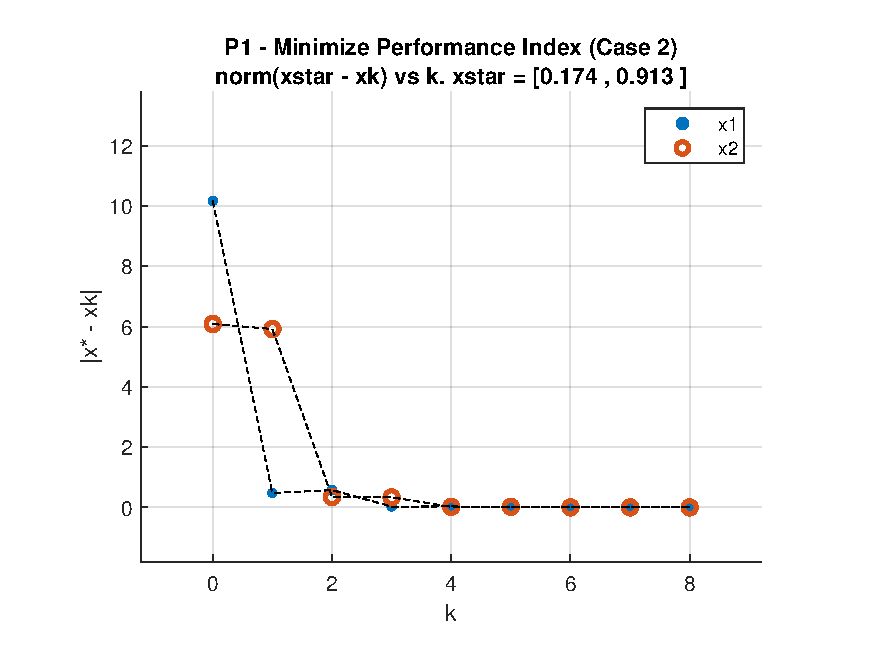
\includegraphics[width=0.8\textwidth]{P1 - Minimize Performance Index (Case 2) - norm(xstar - xk) vs k. xstar = [0.174 , 0.913 ].pdf}
	\end{center}
	\caption{Problem 1: Case 2: Iteration vs. Error}
\end{figure}

% PART THREE 
\subsection{Case 3: x$^0$ = [-2, 14]$^T$}

\subsubsection{Plots}

\begin{figure}[H]
	\begin{center}
		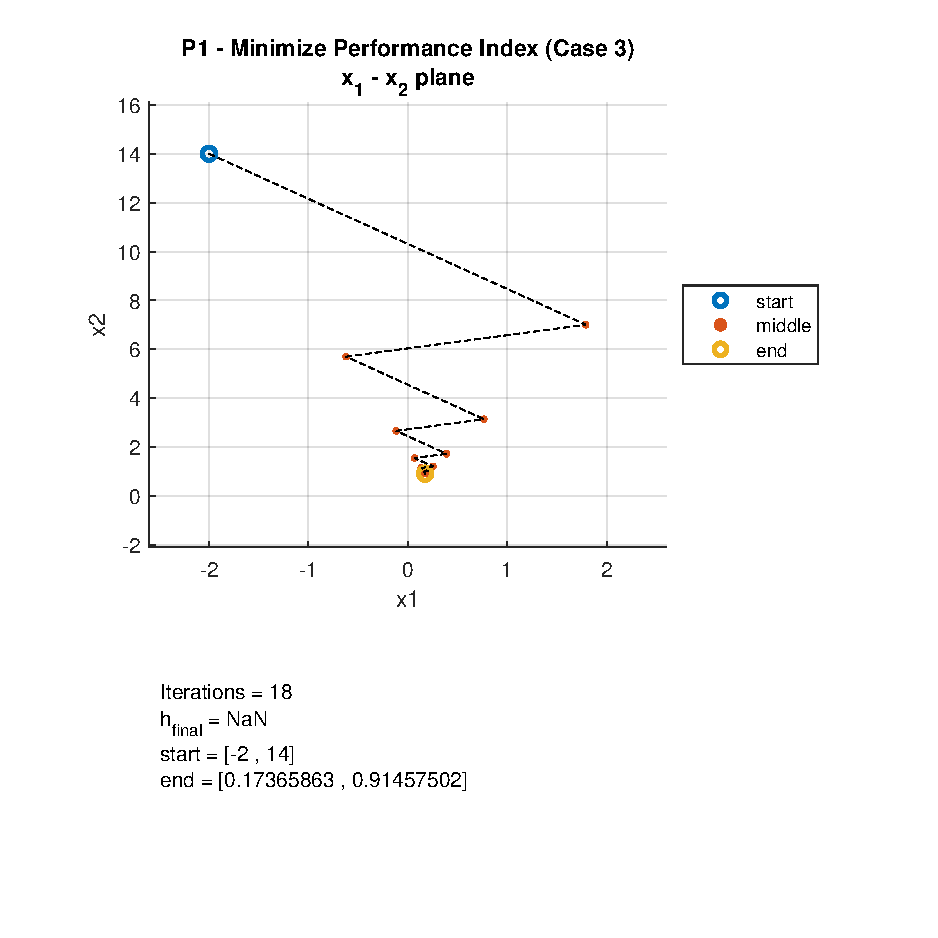
\includegraphics[width=0.9\textwidth]{P1 - Minimize Performance Index (Case 3) - x_1 - x_2 plane.pdf}
	\end{center}
	\caption{Problem 1: Case 3: x1-x2 plane}
\end{figure}

The algorithm took 18 iterations to converge below the threshold $\epsilon = 0.001$. 

\begin{figure}[H]
	\begin{center}
		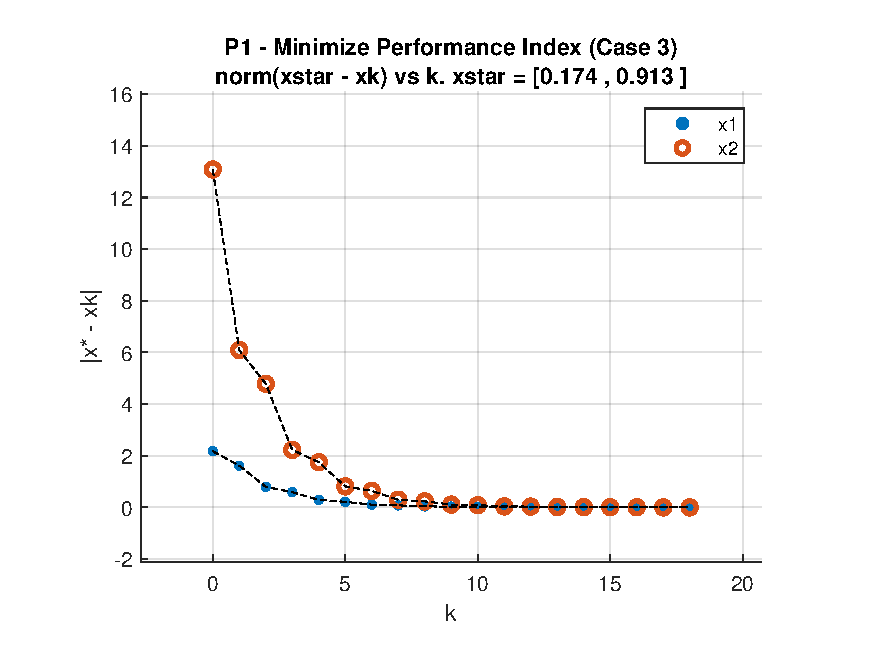
\includegraphics[width=0.8\textwidth]{P1 - Minimize Performance Index (Case 3) - norm(xstar - xk) vs k. xstar = [0.174 , 0.913 ].pdf}
	\end{center}
	\caption{Problem 1: Case 3: Iteration vs. Error}
\end{figure}

% CODE 
\subsection{Code}

\begin{lstlisting}
%% Problem 1 

clear; close all 

% inputs Q and b 
Q = [12 1; 1 2]; 
b = [3; 2];

% analytical solution 
xstar = b' * Q^-1; 

% g function 
g = @(x) Q*x - b; 

% error threshold 
err   = 1e-3; 
delta = 1; 

% FIRST GUESS 
disp('FIRST GUESS')
x0 = [13; -2]; 
[x_arr, i] = min_perf(delta, err, x0, Q, b, g); 

	% plot 1 
	fname1 = 'P1 - Minimize Performance Index (Case 1)'; 
	plot_x1x2(fname1, x_arr, i)
	
	% plot 2 
	plot_xstar_err(fname1, x_arr, xstar, i)        

% SECOND GUESS 
disp('SECOND GUESS') 
x0 = [-10; 7]; 
[x_arr, i] = min_perf(delta, err, x0, Q, b, g); 

	% plot 
	fname1 = 'P1 - Minimize Performance Index (Case 2)'; 
	plot_x1x2(fname1, x_arr, i)
	
	% plot 2 
	plot_xstar_err(fname1, x_arr, xstar, i)

% THIRD GUESS 
disp('THIRD GUESS') 
x0 = [-2; 14]; 
[x_arr, i] = min_perf(delta, err, x0, Q, b, g); 

	% plot 
	fname1 = 'P1 - Minimize Performance Index (Case 3)'; 
	plot_x1x2(fname1, x_arr, i)
	
	% plot 2 
	plot_xstar_err(fname1, x_arr, xstar, i)
	
\end{lstlisting}

\newpage
% ================================================================ % 
\section*{Problem 2}

% Statement 
\begin{center}
	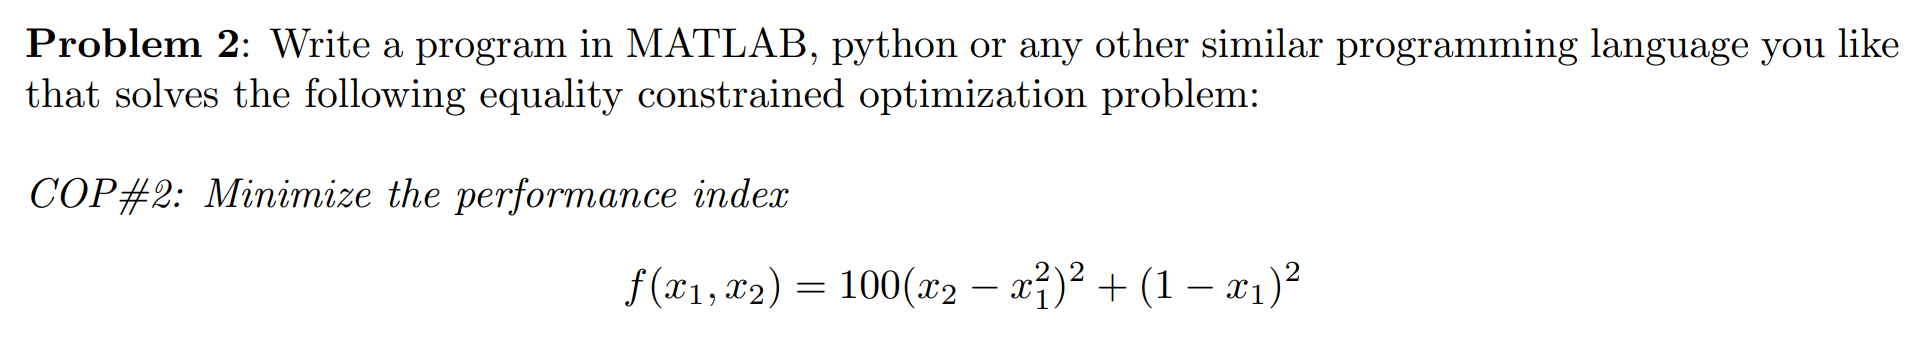
\includegraphics[width=0.9\textwidth]{P2_1.png}
	\vspace{1mm}
	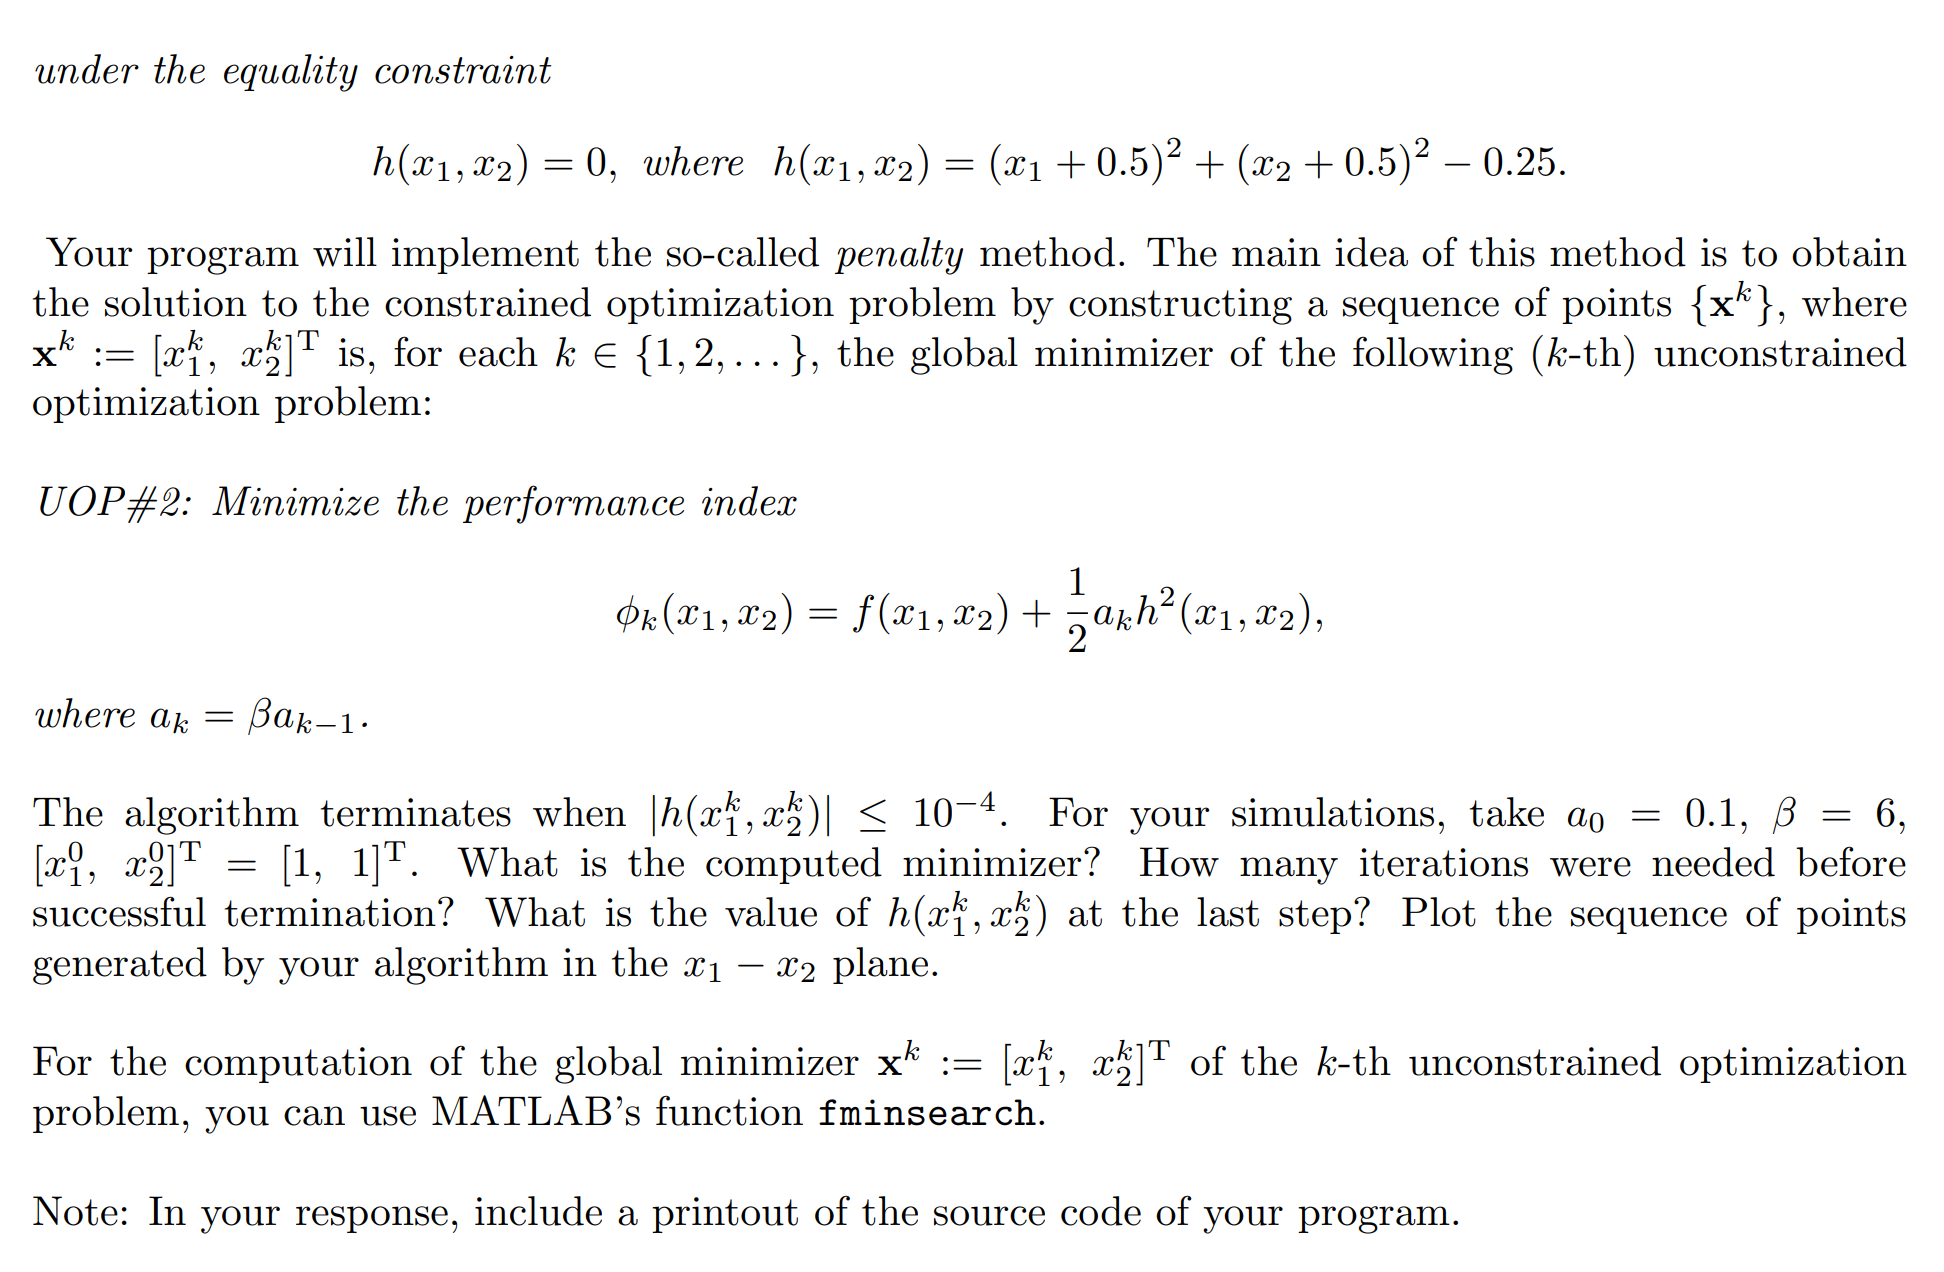
\includegraphics[width=0.9\textwidth]{P2_2.png}
\end{center}


% Solution 

\subsection{Solution}

\begin{figure}[H]
	\begin{center}
		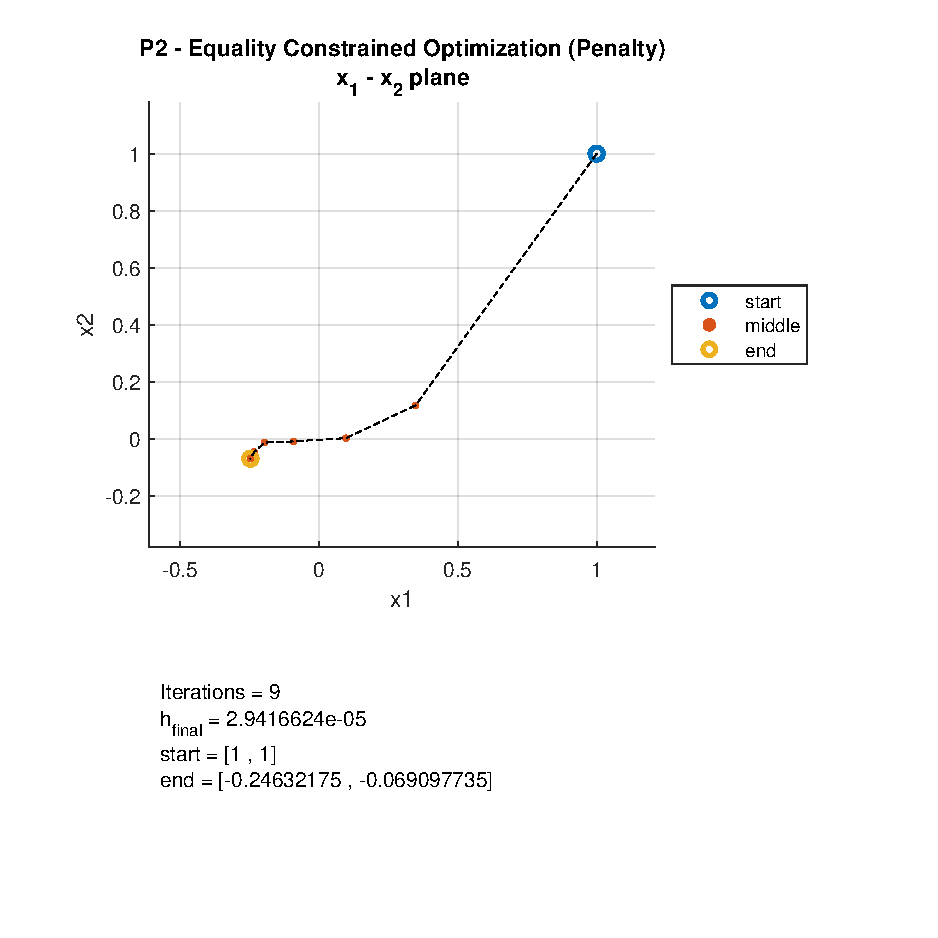
\includegraphics[width=0.9\textwidth]{P2 - Equality Constrained Optimization (Penalty) - x_1 - x_2 plane.pdf}
	\end{center}
	\caption{Problem 2: x1-x2 plane}
\end{figure}

The computed minimizer is [-0.246321750090767, -0.0690977348084581]. The algorithm required 9 iterations before convergence. The value of h at the last step is 2.94166242132965e-05. 

\subsection{Code}

\begin{lstlisting}
%% Problem 2 

clear; 

x = sym('x', [2 1]); 

% create performance index functions 
f = 100 * ( x(2) - x(1)^2 )^2 + ( 1 - x(1) )^2; 
f = matlabFunction(f); 
h = ( x(1) + 0.5 )^2 + ( x(2) + 0.5 )^2 - 0.25; 
h = matlabFunction(h); 

% initialize 
b    = 6;
a0   = 0.1; 
x0   = [1; 1]; 
err  = 10^-4; 

% 0 iteration 
j    = 0; 
akm1 = a0; 
xkm1 = x0; 
h_err = h(xkm1(1), xkm1(2));
x_arr = x0'; 

% iterate 
while h_err > err 
	
	% current index 
	j  = j + 1;  
	ak = b * akm1; 

	phi = @(x) f(x(1), x(2)) + 1/2 * ak * h(x(1), x(2))^2; 
	xk  = fminsearch(phi, xkm1); 
	
	% new penalty 
	h_err = norm(h(xk(1), xk(2))); 
	
	% save output 
	x_arr = [x_arr; xk']; 
	
	% set up next index 
	akm1 = ak; 
	xkm1 = xk; 
	
end 

% plot 
fname1 = 'P2 - Equality Constrained Optimization (Penalty)'; 
plot_x1x2(fname1, x_arr, j, h_err)
\end{lstlisting}

\newpage
% ================================================================ % 
\section*{Problem 3}

% Statement 
\begin{center}
	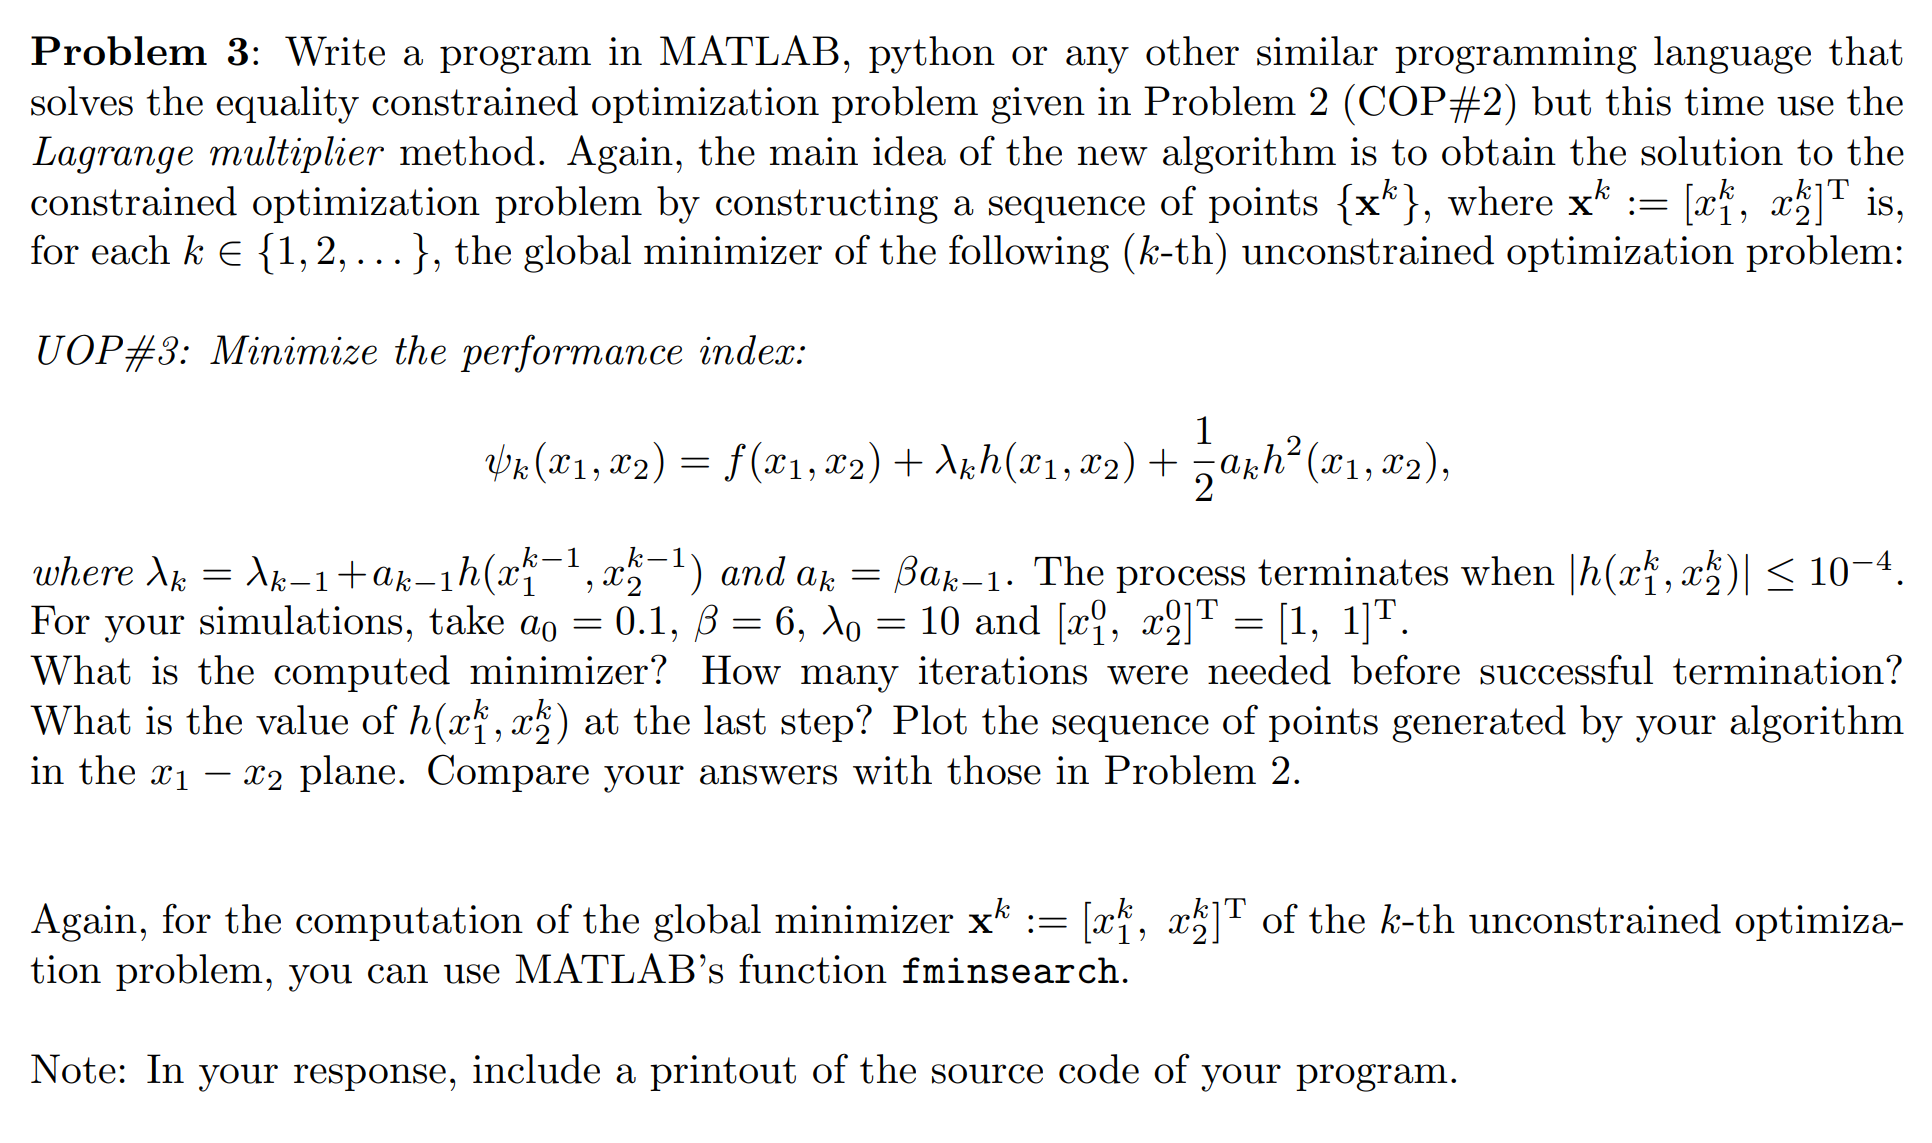
\includegraphics[width=0.9\textwidth]{P3.png}
\end{center}


% Solution 

\subsection{Solution}

\begin{figure}[H]
	\begin{center}
		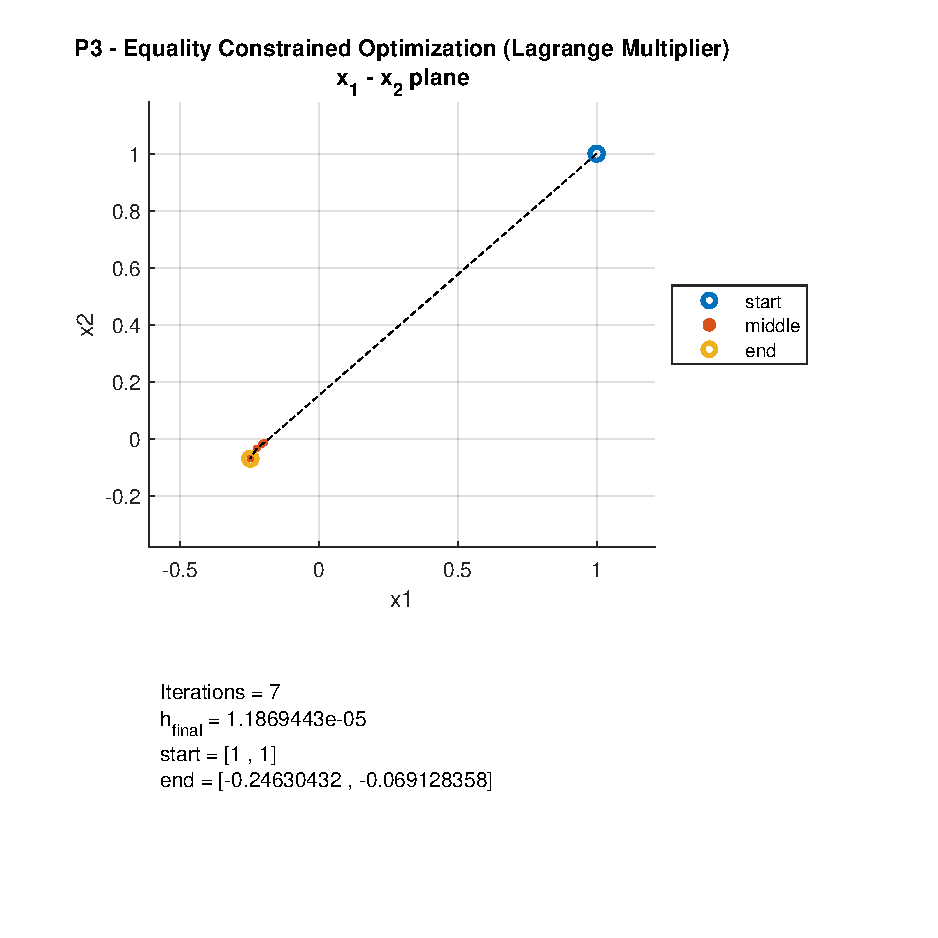
\includegraphics[width=0.9\textwidth]{P3 - Equality Constrained Optimization (Lagrange Multiplier) - x_1 - x_2 plane.pdf}
	\end{center}
	\caption{Problem 3: x1-x2 plane}
\end{figure}

The computed minimizer is [-0.246304320398368, -0.069128358330955]. The algorithm required 7 iterations before convergence. The value of h at the last step is 1.18694431120447e-05. 

The penalty method was used for Problems 2 and 3, but in Problem 3 the Lagrange multiplier method was also implemented. The result is that the Problem 3 algorithm converged more quickly (7 iterations vs. 9) and the penalty value on the final iteration was smaller (1.187e-5 vs. 2.942e-5) than in Problem 2. Additionally, the trajectory of the computed solution at each iteration is straighter and more direct in Problem 3 which can be seen by comparing their plots. The lagrange multiplier method improved the algorithm's performance. 

\subsection{Code}

\begin{lstlisting}
%% Problem 3 

clear; 

x = sym('x', [2 1]); 

% create performance index functions 
f = 100 * (x(2) - x(1)^2)^2 + (1 - x(1))^2; 
f = matlabFunction(f); 
h = (x(1) + 0.5)^2 + (x(2) + 0.5)^2 - 0.25; 
h = matlabFunction(h); 

% initialize 
b    = 6;
a0   = 0.1; 
x0   = [1; 1]; 
err  = 10^-4; 
k    = 0; 
lmda0 = 10; 

% first iteration 
akm1 = a0; 
xkm1 = x0; 
lmdakm1 = lmda0; 
h_err = h(xkm1(1), xkm1(2));
x_arr = x0'; 

% iterate 
while h_err > err 
	
	% current index 
	k     = k + 1; 
	ak    = b * akm1; 
	lmdak = lmdakm1 + akm1 * h(xkm1(1), xkm1(2)); 

	phi = @(x) f(x(1), x(2)) + lmdak * h(x(1), x(2)) + 1/2 * ak * h(x(1), x(2))^2; 
	xk  = fminsearch(phi, xkm1); 
	
	% penalty 
	h_err = norm(h(xk(1), xk(2))); 
	
	% save output 
	x_arr = [x_arr; xk']; 
	
	% set up next index 
	akm1    = ak; 
	lmdakm1 = lmdak; 
	xkm1    = xk; 
	
end 

% plot 
fname1 = 'P3 - Equality Constrained Optimization (Lagrange Multiplier)'; 
plot_x1x2(fname1, x_arr, k, h_err)
\end{lstlisting}


\newpage
% ================================================================ % 
\section*{Appendix} 

\subsection*{Supplementary MATLAB code} 

\begin{lstlisting}
%% subfunctions 

function [x_arr, i] = min_perf(delta, err, x0, Q, b, g) 
% Minimize performance index 

% initialize 
i     = 0; 
x_arr = x0'; 
xkm1  = x0; 

% start iterative process 
while delta > err
	
	% current index 
	i = i + 1; 
	
	% calc ak  
%     ak = ( 1/2 * g(xkm1)' * Q * xkm1 + 1/2 * xkm1' * Q * g(xkm1) - g(xkm1)' * b) * ... 
%         ( g(xkm1)' * Q * g(xkm1) )^-1;     
	ak = inv(g(xkm1)' * Q* g(xkm1)) * (xkm1' * Q * g(xkm1) - g(xkm1)' * b ); 
	
	% calc xk 
	xk = xkm1 - ak * g(xkm1); 
	delta = norm(xkm1 - xk); 
	
	if isnan(delta) 
		disp('Contains NaNs') 
		break
	end 
	
	% save output 
	x_arr = [x_arr; xk']; 
	
	% set up next index 
	xkm1 = xk;

end 

end 

% ------------------------------------------------------------------------ 

function plot_x1x2(fname1, x_arr, k, h_err)

if ~exist('h_err', 'var') 
	h_err = NaN; 
end 
% plot x1-x2 plane 

fname2 = 'x_1 - x_2 plane'; 

figure('name', [fname1 ' - ' fname2], 'position', [100 100 600 600])
	subplot(3,1,1:2) 
		hold on; grid on; 
		scatter(x_arr(1,1), x_arr(1,2), 40, 'linewidth', 2); 
		scatter(x_arr(2:end-1,1), x_arr(2:end-1,2), 10, 'filled')
		scatter(x_arr(end,1), x_arr(end,2), 40, 'linewidth', 2); 
		plot(x_arr(:,1), x_arr(:,2), '--k'); 
		bigger_lim; 

		xlabel('x1'); ylabel('x2'); 
		legend('start', 'middle', 'end', 'location', 'eastoutside')
		title( {fname1; fname2} ); 
	subplot(3,1,3) 
		pos = get(gca, 'position'); 
%         text = {'test1'; 'test2'; 'test3'}; 
		
		text = { ''; ''; 
			sprintf('Iterations = %d', k); 
			sprintf('h_{final} = %.8g', h_err); 
			sprintf( 'start = [%.8g , %.8g]', x_arr(1,1), x_arr(1,2) ); 
			sprintf( 'end = [%.8g , %.8g]', x_arr(end,1), x_arr(end,2) ) }; 
		
		annotation('textbox', pos, ...
			'String', text, ...
			'edgecolor', 'none');
		axis off 
		
end 

function plot_xstar_err(fname1, x_arr, xstar, i)
	
	% plot | xstar - xk |
	dx = abs(x_arr - xstar); 
	fname2 = sprintf('norm(xstar - xk) vs k. xstar = [%.3g , %.3g ]', xstar(1), xstar(2)); 
	figure('name', [fname1 ' - ' fname2] ); 
		hold on; grid on; 
		scatter( [0:1:i]', dx(:,1), 20, 'filled'); 
		scatter( [0:1:i]', dx(:,2), 40, 'linewidth', 2); 
		plot( [0:1:i]', dx(:,1), '--k');         
		plot( [0:1:i]', dx(:,2), '--k'); 
		
		legend('x1', 'x2')
		bigger_lim 
		
		xlabel('k')
		ylabel('|x* - xk|') 
		
		title( {fname1; fname2} ); 

end 

function bigger_lim
% Increase y-axis limits on plot by 30% on current axes 

	ylims       = get(gca, 'ylim'); 
	yrange      = ylims(2) - ylims(1);
	new_ylim    = [ ylims(1) - 0.15*yrange, ylims(2) + 0.15*yrange ]; 
	set(gca, 'ylim', new_ylim);
	
	xlims       = get(gca, 'xlim'); 
	xrange      = xlims(2) - xlims(1); 
	new_xlim    = [ xlims(1) - 0.15*xrange, xlims(2) + 0.15*xrange ]; 
	set(gca, 'xlim', new_xlim); 

end
\end{lstlisting}





% ================================================================ % 

% \bibliography{sample}

\end{document}
